\subsection{Network Science}

A \textit{network} can be thought of as an applied form of a graph \citep{Newman2003} and is generally considered to contain larger sets of vertices and edges in which patterns cannot be easily distinguishable by eye \citep{Newman2003}. Networks often make use of further graph concepts such as \textit{directed edges}, where an edge is associated with a direction \citep{Newman2003}, and \textit{edge weights}, where edges hold some form of value referred to as a \textit{weight} \citep{Bondy1976}. Like graphs, networks can be classified into different types \citep{Newman2003}. For example, a \textit{preference network} is a \textit{bipartite network} (analogous to a bipartite graph) with one partition representing individuals and the second representing objects of interest. The edges between vertices would then denote that an individual has an interest in some object and be weighted according to that interest \citep{Newman2003}. This is demonstrated in Figure \ref{fig:prefnetwork}.

%\afterpage{
    \begin{figure}[t]
        \centering
        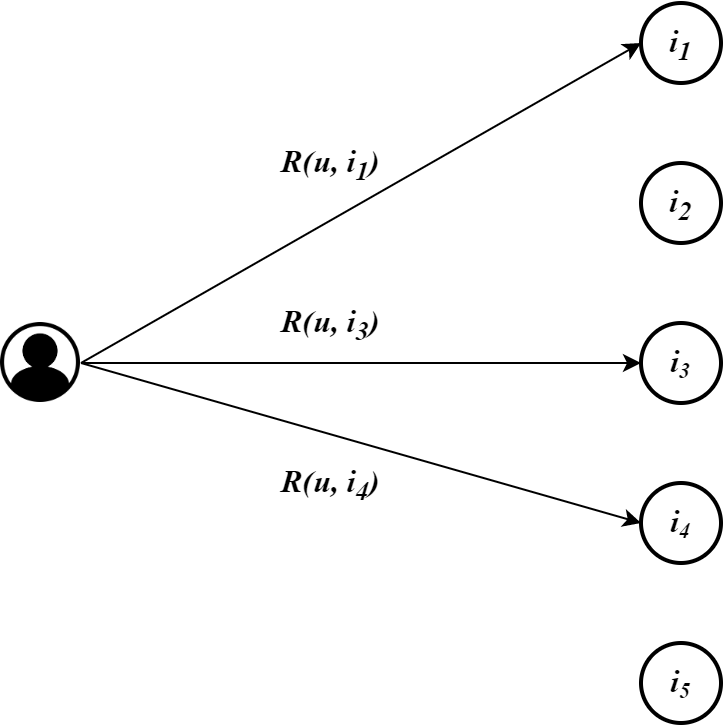
\includegraphics[height = .20\textheight]{preferencenetwork.png}
        \caption{A preference network for a single user represented as a bipartite graph with directed, weighted edges. The left partition holds a single user and the right partition holds items that could be potentially recommended. The edges represent items that will be recommended to the user and the weight of the edges, denoted by the function $R(u, i)$, represents the value of the recommendation \citep{Newman2003}. If an item is not connected to the user by an edge, then it will not be recommended.}
        \label{fig:prefnetwork}
    \end{figure}
%}

Preference networks are the underlying structure behind \textit{recommender systems} \citep{Newman2003}, which are algorithms that provide recommendations to users \citep{Andrews2015}. A \textit{reciprocal recommender system} utilizes the preferences of both the user and the object of interest (typically another user) to determine if they should be recommended to each other \citep{Andrews2015}. For example, such a recommender would not recommend a man who prefers men to a woman who prefers men. In essence, different users have different \emph{utilities} to each other, where utilities represent the value of a recommendation \citep{Andrews2015}. Given a user $u$ and an item $i$ (in this instance, another user), the true utility $R(u, i)$ can be estimated by $\hat{R}(u, i)$ \citep{Andrews2015}. Consider a recommendation system that will recommend $k$ items (referred to as top-$k$ recommendation system \citep{Andrews2015}) given a large set of items denoted 
\begin{equation*}
    \{i_{1}, i_{2}, \ldots i_{n}\}, 
\end{equation*}
where $k \geq 1$, $n \geq 1$, and $k << n$. The system will calculate a set of estimated utilities
\begin{equation*}
    \{\hat{R}(u, i_{1}), \hat{R}(u, i_{2}), \ldots, \hat{R}(u, i_{n})\} ,
\end{equation*}
and then return the top $k$ items with the highest estimated utility. This process is represented in Figure \ref{fig:recalgorithm}.

\begin{figure}[t]
    \centering
    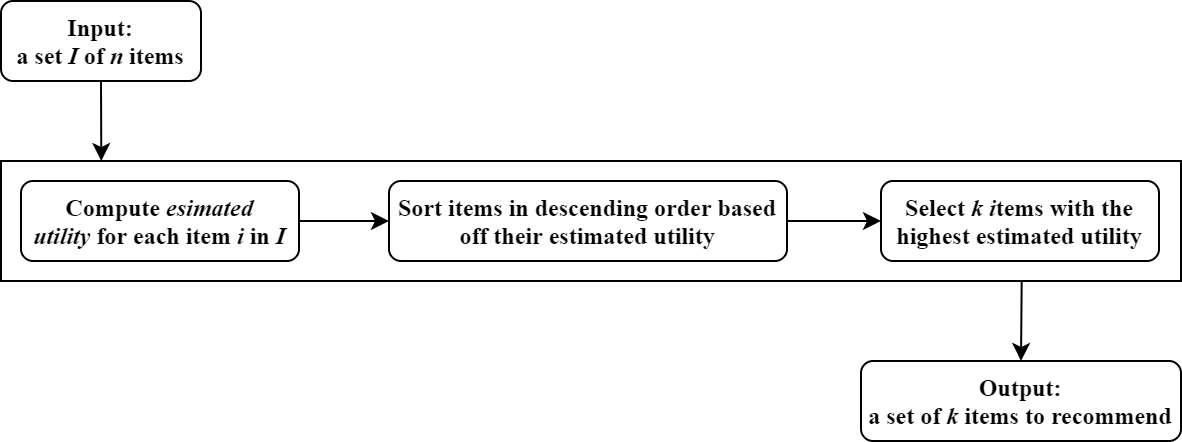
\includegraphics[height = .20\textheight]{recommenderalgorithm.png}
    \caption{A representation of a top-$k$ recommender system. The input is a set of $n$ items and the output is a subset of the input containing the top $k$ items to recommend.}
    \label{fig:recalgorithm}
\end{figure}

If we assume Tinder provides users with recommendations that are meaningful to both the user's goal of forming a relationship and Tinder's goal of maintaining a user base, then $\hat{R}(u, i)$ must factor in the utility of the recommendation to both the two users as well as Tinder itself. For example, a user who will receive a lot of matches but is unlikely to form a relationship with any would have high utility for Tinder. They are not forming relationships with any users, so all users remain in the user base. However, as all users are receiving matches, they are likely to feel more satisfied with the service than if they were receiving no matches at all.

Returning to the preference network, the edge directed from User $A$ to User $B$ would now be weighted by $\hat{R}(A, B)$. In this sense, the edge now holds the direction of preference as well as the ranking of preference. Assuming that Tinder accurately estimates utility relative to the user's own preference, this concept can be used to create a model for Tinder without assuming that users hold equal preferences over each other. However, we will first use this concept to create a model for a generic optimal online dating service instead.